\chapter{System Overview}
\label{chap:sys-overview}

This chapter provides an overview of the system. It presents several
concepts relating to input and output representations, introduces the
four main modules, and discusses how they work together in the
discovery of new definitions and theorems.

\section{Goals}

The end goal of the system is for it to notice and learn interesting
concepts in Geometry from inductive explorations. Because these ideas
are derived from inductive observation, I will typically refer to them
as conjectures. Once the conjectures are reported, they can easily be
integrated into existing automated proof systems if a deductive proof
is desired. The conjectures explored can be grouped into three areas:
definitions, properties, and theorems:

\begin{description}

\enlargethispage*{-\baselineskip}

\item[Properties] Properties include all the facts derived from a
  single premise, such as ``Opposite angles in a rhombus are equal''
  or ``The midpoint of a segment divides it into two equal-length
  segments''.

\item[Definitions] Definitions classify and differentiate an object
  from other objects. For instance ``What is a rhombus?'' yields the
  definition that it is a quadrilateral (classification) with four
  equal sides (differentiation). As seen in the demonstration, the
  system will attempt to simplify definition properties to more
  minimal sets, provide alternative formations, and use pre-existing
  definitions when possible: ``A square is a rhombus and a rectangle''

\item[Theorems] Theorems involve relations among additional elements
  constructions from an initial premise. For instance, theorems about
  triangles may involve the construction of angle bisectors, incenters
  or circumcenters, or the interaction among several polygons in the
  same diagram.

\end{description}

Given a repository of these conjectures about geometry, the system
will be able to apply its findings in future investigations by
examining elements to display its knowledge of definitions, and
focusing future investigations by omitting results implied by prior
theorems.

\section{Diagram Representations}

The system and modules are built around three core diagram
representations. As discussed in the motivation section, we use the
term ``diagram'' to represent the abstract geometric object
represented by these means:

\begin{description}

\item[Construction Steps] The main initial representation for most
  diagrams is a series of construction steps. These generally comprise
  the input investigation from an external user trying to teach the
  system a concept. In some investigations, the actual construction
  steps are opaque to the system (as in a teacher that provides a
  process to ``magically'' produce rhombuses), but often, the
  construction steps use processes known by the system so that the
  resulting figures can include dependency information about how the
  figure elements are built.

\item[Analytic Figure] The second representation is an analytic figure
  for a particular instance of a diagram. This representation includes
  coordinates for all points in the diagram and can be displayed. This
  representation is used by the perception module to observe
  interesting relationships.

\item[Symbolic Relationships] Finally, the third representation of a
  diagram is as a collection of symbolic relationships or constraints
  on elements of the diagram. These are initially formed from the
  results of the perception module, but may also be introduced as
  known properties for certain premises and construction steps. These
  symbolic relationships can be further tested and simplified to
  discover which sets of constraints subsume one another.

\end{description}

While construction steps are primarily used as input and to generate
examples, as the system investigates a figure, the analytic figure and
symbolic relationship models get increasingly intertwined. The ``mind's
eye'' perception aspects of observing relationships in the analytic
figure lead to new symbolic relationships and a propagator-like
approach of wigging solutions to the symbolic constraints yields new
analytic figures.

As relationships are verified and simplified, results are output and
stored in the student's repository of geometry knowledge.


\section{Steps in a Typical Interaction}

The system overview figure on the next page depicts the typical
process of interacting with the system and shows relationships between
the four system modules.

These four modules are an imperative geometry construction interpreter
used to build diagrams, a declarative geometry constraint solver to
solve and test specifications, an observation-based perception module
to notice interesting properties, and a learning module to analyze
information from the other modules and integrate it into new
definition and theorem discoveries.

\newpage

\begin{figure}[h!]
\centering
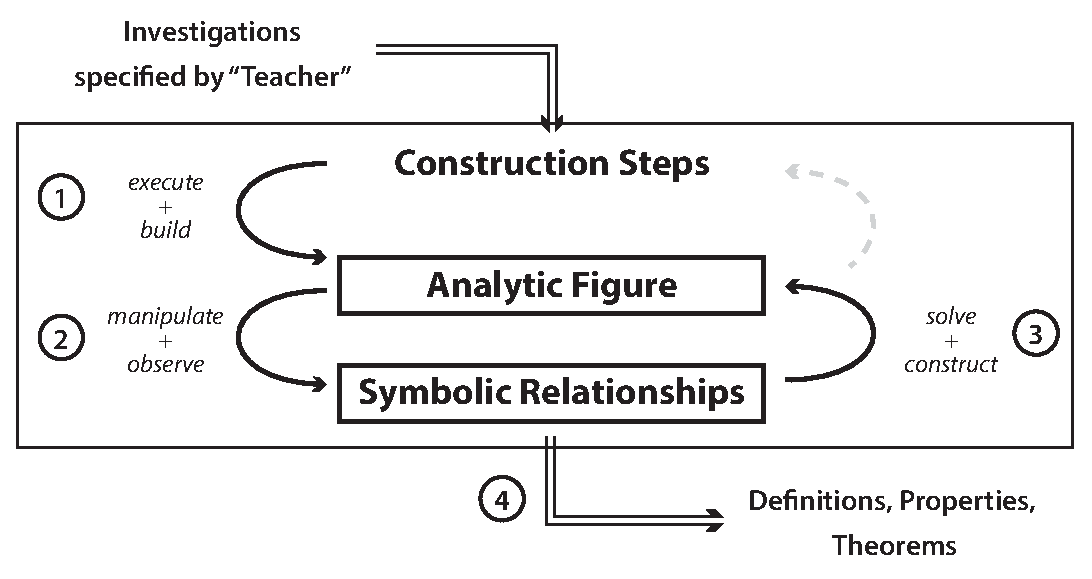
\includegraphics[width=0.9\textwidth]{diagrams/Representations.eps}
\captionsetup{labelformat=empty}
\caption{{\bf System Overview:} Given construction steps for an
  investigation an external teacher wishes the student perform, the
  system first (1) uses its imperative construction module to execute
  these construction steps and build an analytic instance of the
  diagram. Then, (2) it will manipulate the diagram by ``wiggling''
  random choices and use the perception module to observe interesting
  relationships. Given these relationships, it will (3) use the
  declarative propagator-based constraint solver to reconstruct a
  figure satisfying a subset of the constraints to determine which are
  essential in the original diagram. Finally (4), a learning module
  will monitor the overall process, omit already-known results, and
  assemble a repository of known definitions, properties, and
  theorems.}
\end{figure}

\subsection{Interpreting Construction Instructions}

\enlargethispage*{\baselineskip}

The first step in an exploration is interpreting an input of the
diagram to be investigated.  The imperative construction module takes
as input explicit construction steps that results in an instance of
the desired diagram.  These instructions can still include arbitrary
selections (let $P$ be some point on the line, or let $A$ be some
acute angle), but otherwise are restricted to basic construction
operations that could be performed using a compass and straight edge.

To simplify the input of more complicated diagrams, some of these
steps can be abstracted into a library of known construction
procedures.  For example, although the underlying figures are limited
to very simple objects of points, lines, and angles, the steps of
constructing a triangle (three points and three segments) or bisecting
a line or angle are encapsulated into single steps.

\subsection{Creating Figures}

Given a language for expressing the constructions, the second phase of
the system is to perform such constructions to yield an instance of
the diagram.  This process mimics ``imagining'' images and results in
an analytic representation of the figure with coordinates for each
point.  Arbitrary choices in the construction (``Let $Q$ be some point
on the line.'') are chosen via an random process, but with an attempt
to keep the figures within a reasonable scale to ease human
inspection.

\subsection{Noticing Interesting Properties}
\label{sec:interest}

Having constructed a particular figure, the system examines it to find
interesting properties.  These properties involve facts that appear to
be ``beyond coincidence''.  This generally involves relationships
between measured values, but can also include ``unexpected''
configurations of points, lines, and circles.  As the system discovers
interesting properties, it will reconstruct the diagram using
different choices and observe if the observed properties hold true
across many instances of a diagram.

\subsection{Reporting and Simplifying Findings}

Finally, once the system has discovered some interesting properties
that appear repeatedly in instances of a given diagram, it reports its
results to the user via the learning module.  Although this initially
includes a simple list of all simple relationships, effort is taken to
avoid repeating observations that obvious in the construction.  For
example, if a perpendicular bisector of segment $AB$ is requested, the
fact that it bisects that segment in every instance is not
informative.  To do so, the construction process interacts with
properties known in the learning module to maintain a list of facts
that can be reasoned from construction assumptions so that these can
be omitted in the final reporting. Finally, given several properties
true of a figure, the learning module uses the constraint solver in an
attempt to reconstruct a figure satisfying a subset of the constraints
to determine which are essential in the original diagram.
